%%%%%%%%%%%%%%%%%%%%%%%%%%%%%%%%%%%%%%%%%%%%%%%%%%%%%%%%%%%%%%%%%%%%%%%%%%%%%%%%
% Template for USENIX papers.
%
%%%%%%%%%%%%%%%%%%%%%%%%%%%%%%%%%%%%%%%%%%%%%%%%%%%%%%%%%%%%%%%%%%%%%%%%%%%%%%%%
\documentclass[letterpaper,twocolumn,10pt]{article}
\usepackage{usenix}

% to be able to draw some self-contained figs
\usepackage{tikz}
\usepackage{amsmath}
\usepackage{xxxnotes}

% inlined bib file
\usepackage{filecontents}

%-------------------------------------------------------------------------------
\begin{filecontents}{\jobname.bib}
%-------------------------------------------------------------------------------
@incollection{positiongdpr,
  title={Position: Gdpr compliance by construction},
  author={Schwarzkopf, Malte and Kohler, Eddie and Kaashoek, M Frans and Morris, Robert},
  booktitle={Heterogeneous Data Management, Polystores, and Analytics for Healthcare},
  pages={39--53},
  year={2019},
  publisher={Springer}
}
\end{filecontents}

%-------------------------------------------------------------------------------
\begin{document}
%-------------------------------------------------------------------------------

\date{}

% make title bold and 14 pt font (Latex default is non-bold, 16 pt)
\title{\Large \bf Designing GDPR Compliant-by-Construction Systems}

%for single author (just remove % characters)
\author{
{\rm Lillian Tsai}\\
MIT
% copy the following lines to add more authors
% \and
% {\rm Name}\\
%Name Institution
} % end author

\maketitle

%-------------------------------------------------------------------------------
\section{Introduction}
%-------------------------------------------------------------------------------
Websites such as Facebook, Twitter, and Google have historically controlled the storage and processing of their users' data.
A user uploading data to such services would forfeit the right to control that data, allowing the website to dispense and retain her data, perhaps indefinitely.
With the recent introduction of the European Union's General Data Protection Regulation (GDPR) laws, 
users gain explicit rights to own their data: they have the right to obtain, as well as completely erase, 
any of their data stored by the service. 
However, implementing GDPR-compliant services is not straightforward, 
as current system designs were not designed with user data ownership as a first principle.

This paper introduces a design and prototype for a new data storage model loosely based upon the one proposed by Schwarzkopf et al.~\cite{positiongdpr}, 
which suggests new abstractions for GDPR compliant-by-construction systems. 
In this model, each end-user of a web service maintains their own mini-database (a ``user shard'') 
that holds all information pertaining to them and related to this service. 
The data available to the shared service is the cumulative sum of all the underlying user shards, which the service can combine and process. 
Each user grants the service a lease to the data in their shard, permitting the service to store and compute over this data. 
The service promises to remove the provided data and any derived computation when the lease is revoked.
This model of data storage raises many questions that this project aims to investigate:
\begin{itemize}
    \item What is the impact of logically (or physically) disjoint user data? How will the movement of data from user-owned shards to shared storage affect service load and throughput?
    \item What does it mean to "own" data in the context of a specific web application? For example, who owns a private messaging conversation on Facebook, or a reply made on Twitter?
        How do different "ownership" policies affect the semantics and performance of these web applications?
\end{itemize}

%-------------------------------------------------------------------------------
\section{System Design}
%-------------------------------------------------------------------------------
The system model consists of two components: 
(1) end-user clients, each with a user shard (mini-database) that contains that specific user's data; 
(2) a shared service with access to the cumulative sum of all user shards, with the ability to combine and process this data.
Users subscribe to and update the service via RPC calls (see Section~\ref{sec:rpcs}).
Figure~\ref{fig:design} shows the flow of data through the system.

\begin{figure}
    \centering
    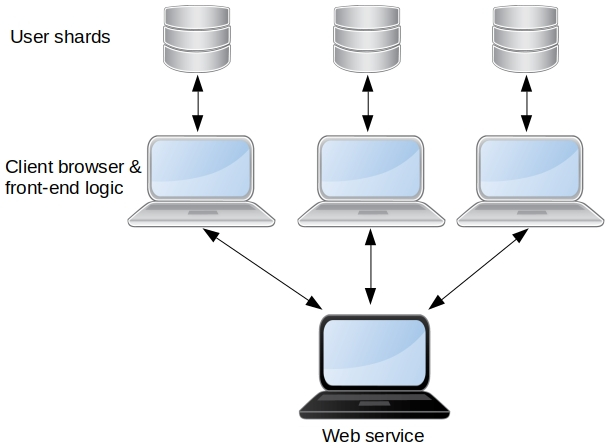
\includegraphics[width=0.4\textwidth]{usershards}
    \caption{Clients privately store and update data in user shards, and send updates to a shared web service. Clients can then read (potentially processed) data from the web service.}
    \label{fig:design}
\end{figure}

A client must be aware of the objects manipulated by the service (e.g., posts, comments, photos, etc.) 
in order to correctly send shard data updates to the service. A user shard is inaccessible by the service or other users; 
this could be stored either locally on the client itself or in a Cloud storage system such as AWS, 
depending on the privacy requirements of the user, the amount of user data, and
the cost the user (or service) is willing to pay.

While data flows explicitly between client and service via RPC calls, 
the service can only retain data if the user grants the service a \emph{lease}
to the data. Our design associates an expiration time with each user's lease for her data, after
which the lease is implicitly revoked; the user can also explicitly revoke the lease.
When a lease is revoked, the user's data is removed from the service.
We describe leases in further detail in Section~\ref{sec:leases}. 
While automatic data revocation goes beyond the requirements of the GDPR, we include 
leases in order to strengthen the notion of user data ownership. Indeed, services such as Google 
support automatic revocation of user data after a specified period of nonuse.

\subsection{RPC Interface}
\label{sec:rpcs}
RPCs between client and service fall into three classes of operations:
\begin{enumerate}
    \item shard management operations
    \item write operations (insertions, modifications, deletions)
    \item read operations
\end{enumerate}

User shard management operations include operations such as \texttt{subscribe} and \texttt{unsubscribe}. 
A \texttt{subscribe} operation establishes a connection with the service if one does not exist, and contains all data and writes that the service has not received from the client. This may include writes that were logged but not yet sent to the service (see Section~\ref{sec:logging}) due to a crash, or data that had been revoked due to a lease expiration (see Section~\ref{sec:leases}) or \texttt{unsubscribe} operation (\texttt{unsubscribe} removes all user data from the service).

%While unsubscribed, the client refuses any updates that occur while unsubscribed: this ensures that writes appear consistently to every user, i.e., 
%users only receive successful responses when the change has been reflected by the service and is visible to others.
%This prevents, for example, a situation in which a user issues a (successful) delete-post request while its client is unsubscribed, but another subscribed client adds comments onto the not-yet-removed post.
Write and read operations are implemented in an application-specific manner.
For example, a social network service may include write operations to create new posts,
delete posts, make comments, or edit post text.

\subsection{Consistency Model}
\label{sec:logging}
For every write, the client first sends the RPC to the service, and then only applies the write to the user shard if the RPC succeeded. 
Alternatively, the client could also apply the write to the user shard, then 
send an RPC to the service and waits for a successful reply.
With either approach, we preserve the invariant that the shared service is the 
cumulative sum of the clients' user shards.

We note that the service's application order determines the linearization point of the operation.
For example, if one client deletes a post, and another client concurrently comments on the post,
the service can either apply the deletion first and return \texttt{error} to the commenter, or post the comment first
and return \texttt{success}.

In order to ensure that writes provide a consistent view to all users even in the face of disconnects or crashes 
while RPCs are in flight, the client implements a persistent write-ahead-log (WAL). 
Prior to applying the write to its database and sending the service an RPC, the client logs the write information; 
the log entry is marked committed (so the log may later be truncated) when the client write receives a successful RPC reply. 
During recovery from failure or upon subsequent \texttt{subscribe}s, the client issues any uncommitted writes remaining in the log. 
Both service and client-side code must ensure that these writes are either idempotent, or detect duplicate requests via 
monotonically increasing identifiers for every write (not applying any write with a identifier lower than that of the last applied write); our design
does the latter.

In order to improve performance, the system can perform writes in batches: instead of every update generating two disk writes, every batch of writes would generate two disk writes. 
To allow for reads to proceed even when writes are batched, this may require weakening the consistency model such that reads can observe state prior to any write that has returned but been batched. 
Or perhaps there can be client-side read-my-writes resolution; however, the client may not necessarily have enough information to know how these writes would be processed by the service.
%\XXX{I actually don't see any read-my-writes issues here---the client won't be able to proceed with a subsequent read until 
%a write has been both processed by the service and the user shard. 
%If we were to implement batching, it seems like any client read would require that all batched writes be issued and acknowledged by the service before the read returns, because the client wouldn't necessarily have enough information to know how the service
%would process all writes. Am I forgetting something trivial here?}

\subsection{Lease Revocation}
\label{sec:leases}
A user's data is associated with a \emph{lease}; while the service holds the lease, it may process and share a user's data. 
Lease renewals occur when a user contacts the service: users may send heartbeats (empty update RPCs), a normal update, a read request,
or simply resubscribe to the service.
Unless otherwise specified, user leases are automatically revoked after 5 years of non-renewal.  

For simplicity, our prototype design enforces coarse-grained leases: the lease applies to all of the user's data.
We can also imagine an alternative design, in which every piece of user data has a separate lease; however, this complicates the system design, 
as either (or both) the user and the service must track individual leases for potentially hundreds or thousands of distinct pieces
of data. However, given particular service applications, this lease design may be inevitable: for example, users may wish to 
lease their post data for a shorter period of time than their likes on posts.

Given this lease design, the service must ensure that it removes all user data 
from its local storage when the lease time is up.
If the user issues any RPCs after the lease has expired, 
the service will need to re-request all user data,
and will notify the user by returning an error code.
The user will then issue a \texttt{subscribe} request with the required data.

\subsection{Basic Data and Revoking Data Effects}
Because one user's data can affect many derived pieces of data in the service (such as an aggregate vote count), and other users' data may be semantically dependent upon one user's data (such as comments on the user's posts),
revoking one user's data can raise thorny questions about how to handle other related data written by other users.
For example, what will happen if a comment is made on a post that another user deletes? Should the comment be removed? Or does this comment belong to the user who posted it? 

Our design takes the stance that whatever a user writes---contains in their user shard---is owned by the user.
We maintain the invariant that if user data is deleted (either via lease revocation or through a delete request), the service
will no longer store that data. We call data objects directly corresponding to data in the user's shard \emph{basic data}.

Basic data generates \emph{effects} throughout the service: these effects can be derived data, such as a vote count, or dependent data owned by other users, such as comments.
In our design, the service specifies an \emph{effect deletion policy} per type of basic data (e.g., one policy for votes, and one policy for posts) that determines how to deal with the effects of basic data that are deleted.
The three types of effect deletion policies are as follows:
\begin{enumerate}
    \item \textbf{Retain Effects}: The basic data is deleted from the service, but all effects of the basic data remain visible and accessible to all users. For example, the removal of a vote would not affect the vote count; the removal of a post would anonymize and delete the post content, still allow users to see the associated comment chain.
    \item \textbf{Revoke+Store Effects}: The basic data is deleted from the service, and all effects of the basic data are made inaccessible to all users. However, the service may still store the effects of the basic data in its storage. For example, the vote count would change when a vote is removed; a comment chain would be made inaccessible (but still kept in the application's storage) when the parent post is removed.
    \item \textbf{Revoke+Delete Effects}: The basic data and all effects of the basic data are deleted from the service. For example, the vote count would change when a vote is removed; all comments beneath a delete post would be deleted from service storage.
\end{enumerate}

Each of these policies presents a different set of benefits and challenges during both user data deletion and (re)insertion. We outline some of these in the context of a service with votes, comments (potentially nested), and posts as the basic data; and vote counts and comment chains as the ``effects'' of these basic data.
We see that the complexity of each policy for different basic data depends on whether the data has \emph{idempotent} and/or \emph{deterministic} effects. 

\paragraph{Retaining Effects.}
Retaining the effects of basic data, simplifies basic data deletion but potentially complicates inserts for basic data with \emph{non-idempotent} effects.
When basic data is removed, the service does not need to modify any effects: in our example, the vote count remains unmodified, and the comment chain remains intact. The service needs only remove (and anonymize) any trace of the basic data content: in this example service, votes are deleted from service storage, and
posts or comments are anonymized and their textual content removed.

However, the service must ensure that reinserting deleted basic data does not duplicate any effects: if the effect is non-idempotent (applying the effect more than once leads to a different final state than applying it once), the service must remember that the effect has already been applied.
For example, the reinsertion of a vote must not change the vote count if the vote had previously been deleted.
This requires the service to remember any deleted basic data that generate non-idempotent effects in order to distinguish if a vote sent via a user write had previously been deleted, or is a new vote, and update the vote count accordingly.

In contrast, inserting a post or comment has an idempotent effect, namely filling a specific link in a specific comment chain. Thus, the service does not need to remember deleted posts or comments.

Depending on the service and basic data, retaining the effects of basic data can allow for more sensible service behavior. For example, applications such as 
Reddit allow for users to see their comments on posts that may have been deleted.
Or if votes are only positive, then users can boast that their posts received "1 million upvotes" without the fear that this count may decrease.

\paragraph{Revoking Effects.}
Revoking the effects of basic data makes the effects inaccessible to any other user. 
We provide two options when a service revokes effects: the service can keep the effects stored, or must delete them from storage.
Keeping the effects allows the service to easily restore effects if the basic data is re-inserted; otherwise, the service would be required to \emph{pull} data from other user shards. 
For example, if the service deleted an entire comment chain when a post is removed, the service 
would have to re-query all users who commented in the chain for the relevant comments.
(Note that for effects such as vote count, restoring the effect is much simpler: inserting a vote simply updates the vote count).

For basic data such as votes, revocation policies are actually simpler than retention policies: 
the deletion and insertion of a vote simply modifies the vote count accordingly.
This simple implementation arises from the fact that the effects of votes (i.e., vote count in this service) are \emph{deterministic}: 
the service can apply a function on insert to apply the effect, and its inverse on deletion to make the effect inaccessible.

However, the effect of posts and comments---namely comment chains---depend on the actions of other users, and vary from post to post.
In order to make all comments in the comment chain below a deleted post inaccessible, but still keep these comments in service storage, the service recursively encrypts the ID (including the authoring user ID) of each comment using a secret key known only to the service, deletes 
the original comment, and stores the encrypted ID and comment content in storage.
The encrypted ID ensures that no user can query for an inaccessible comment. 
The encrypted ID also allows the service to authorize users to delete currently inaccessible comments from service storage; 
this is necessary to preserve the invariant that
all deleted basic data objects are deleted from service storage.
The service can later recursively restore the comment chain if the parent post or comment is reinserted.

If the service had deleted, rather than encrypted, all dependent comments below a reinserted parent, then the service would have to re-query all users for these comments in the chain. Alternatively, the service could provide no promise to users that their comments will remain on chains or posts that have been deleted and then reinserted, which seems semantically problematic (a user could rewrite comment chain history by simply 
deleting and reinserting). 

The complexity of revoking effects of comments or posts arises from the fact that these effects are nondeterministic: they cannot be restored without the service remembering some amount information. Furthermore, this information must be stored in an inaccessible way.

As with retaining effects, revocation policies can make more or less sense depending on the service and basic data. For example, Facebook or Instagram removes access to comment chains on deleted photos, and like counts fluctuate as users delete their accounts or likes.

%-------------------------------------------------------------------------------
\section{Implementation and Evaluation}
%-------------------------------------------------------------------------------
We provide a prototype of our design written in Go. Each user shard is represented as a MySQL database, and the service stores copies of user shards as well as materialized views over all user data in an in-memory hashtable. Each client owning a user shard communicates via Go RPCs with the service, which is currently implemented as a non-fault-tolerant single machine.
When users start (or restart after a crash), they recover by issuing any entries in their log to both their database and the service.

The service is a simple news-feed type application. The basic data includes articles, comments (on articles or comments), and up- or down-votes (on articles or comments). The service keeps track of effects of the basic data, namely comment chains and aggregate up- or down-vote counts. Users can insert, modify, and delete their basic data; each piece of basic data has a unique identifier as well as a version to allow for updates to be properly ordered and identified.
The version also prevents duplicate writes, and can be used to detect whether the user and service are properly synced.
Users can read articles or comments (along with their vote counts) by querying the unique ID for the article or comment.

Each type of basic data comes with an effect deletion policy, which is passed into the service via initialization arguments. Our service implements each deletion policy as described above; however, the current implementation of ``Revoke+Delete'' does not pull comments from user shards after reinsertion (sacrificing semantics for simplicity and performance).

We perform several experiments to evaluate our driving performance questions:
\begin{itemize}
    \item How will the movement of data from user-owned shards to shared storage affect service load and throughput?
    \item How do different "ownership" policies affect the performance of these web applications?
\end{itemize}
Our experiments generate sets of data representing each user's shard; the amount of data each user shard contains is sampled from a Zipf distribution (parameter 2.75). This models a system in which many users are passive or low-activity, and a few users are "super-user". 
We ensure that a specific user $U$ is a super-user, generating 100K articles, 500K comments, and 1 million votes for this $U$'s user shard.

For the duration of the test (2 minutes), up to 100 users run a mix of deletions, updates, and reads every $t$ ms, where $t$ ranges from 10 to 100ms. $U$ switches phase from subscribed to unsubscribed, and vice versa, after a phase duration has passed (20 seconds).
We then measure the effect of an unsubscription (or lease revocation) and resubscription by $U$ by measuring the impact on the service's throughput (time for other users' requests to be serviced) and load (number of writes the service performs). We test these effects for the three different effect deletion policies.
As a baseline, we simply stop the execution of $U$ during the duration of the ``unsubscribed'' phase, but do not issue any revocations or reinsertions to the service.

Our preliminary results indicate that, as expected (with this simple schema), the number of extra writes of the service generated when $U$ subscribes or unsubscribes is linear in the number of basic data records in $U$'s user shard.

Our baseline results for a "retain" policy indicates that reads take on average ~0.5s (ranging 0.45-0.7s), while updates (inserts and deletions) of both votes and texts take on average ~90s (ranging 86-94s).
We see no increase for read latency when $U$ unsubscribes and subscribes, but we do observe an increase in update latency to an average of 97s (with a max of 111s).

Our baseline results for a "revoke+delete" policy has similar performance for reads, while updates (inserts and deletions) of both votes and texts take slight longer on average (~95s, ranging 94-105s).
Again, we see no increase for read latency when $U$ unsubscribes and subscribes, but we do observe an enormous increase in update latency (both average and variance) to an average of ~150s (ranging from 97-244s).

%-------------------------------------------------------------------------------
\section{Conclusion and Future Work}
We propose a design and implement a prototype for a GDPR compliant-by-construction system, where users maintain separate user shards, and a shared service is granted only temporary access to user data. Our design discusses various policies for how such a service should handle data lease revocations and deletions of user data. In particular, we see that different policies can have drastically different implications for the semantics and performance of the service.

We aim to continue the project far beyond what is discussed here. Our first step is to collect more performance statistics for the initial implementation, and pinpoint and optimize the performance bottlenecks for each deletion policy. 
To improve overall performance, we also plan to implement log entry batching and handling read-my-writes with this scheme, as well as log checkpointing.

As the project progresses, we aim to support a more complex and interesting schema, and explore automation of the implementation of various effect deletion policies for general classes of basic data objects.
%\XXX{Fault tolerance/replication in the shared service?}
%\XXX{Make the schemas/queries supported more complex}

\section{Acknowledgements}
This project (currently just in a budding stage) would not have been possible without the guidance by Malte Schwarzkopf, Eddie Kohler, and Robert Morris; their patience and insights have been invaluable, and I look forward to collaborating on this project as it develops. 

%-------------------------------------------------------------------------------
%-------------------------------------------------------------------------------

\bibliographystyle{plain}
\bibliography{\jobname}

%%%%%%%%%%%%%%%%%%%%%%%%%%%%%%%%%%%%%%%%%%%%%%%%%%%%%%%%%%%%%%%%%%%%%%%%%%%%%%%%
\end{document}
%%%%%%%%%%%%%%%%%%%%%%%%%%%%%%%%%%%%%%%%%%%%%%%%%%%%%%%%%%%%%%%%%%%%%%%%%%%%%%%%
%%  LocalWords:  endnotes includegraphics fread ptr nobj noindent
%%  LocalWords:  pdflatex acks
